\section{Internal implementation}

\subsection{Overall architecture}

\begin{figure}[H]
    \centering
    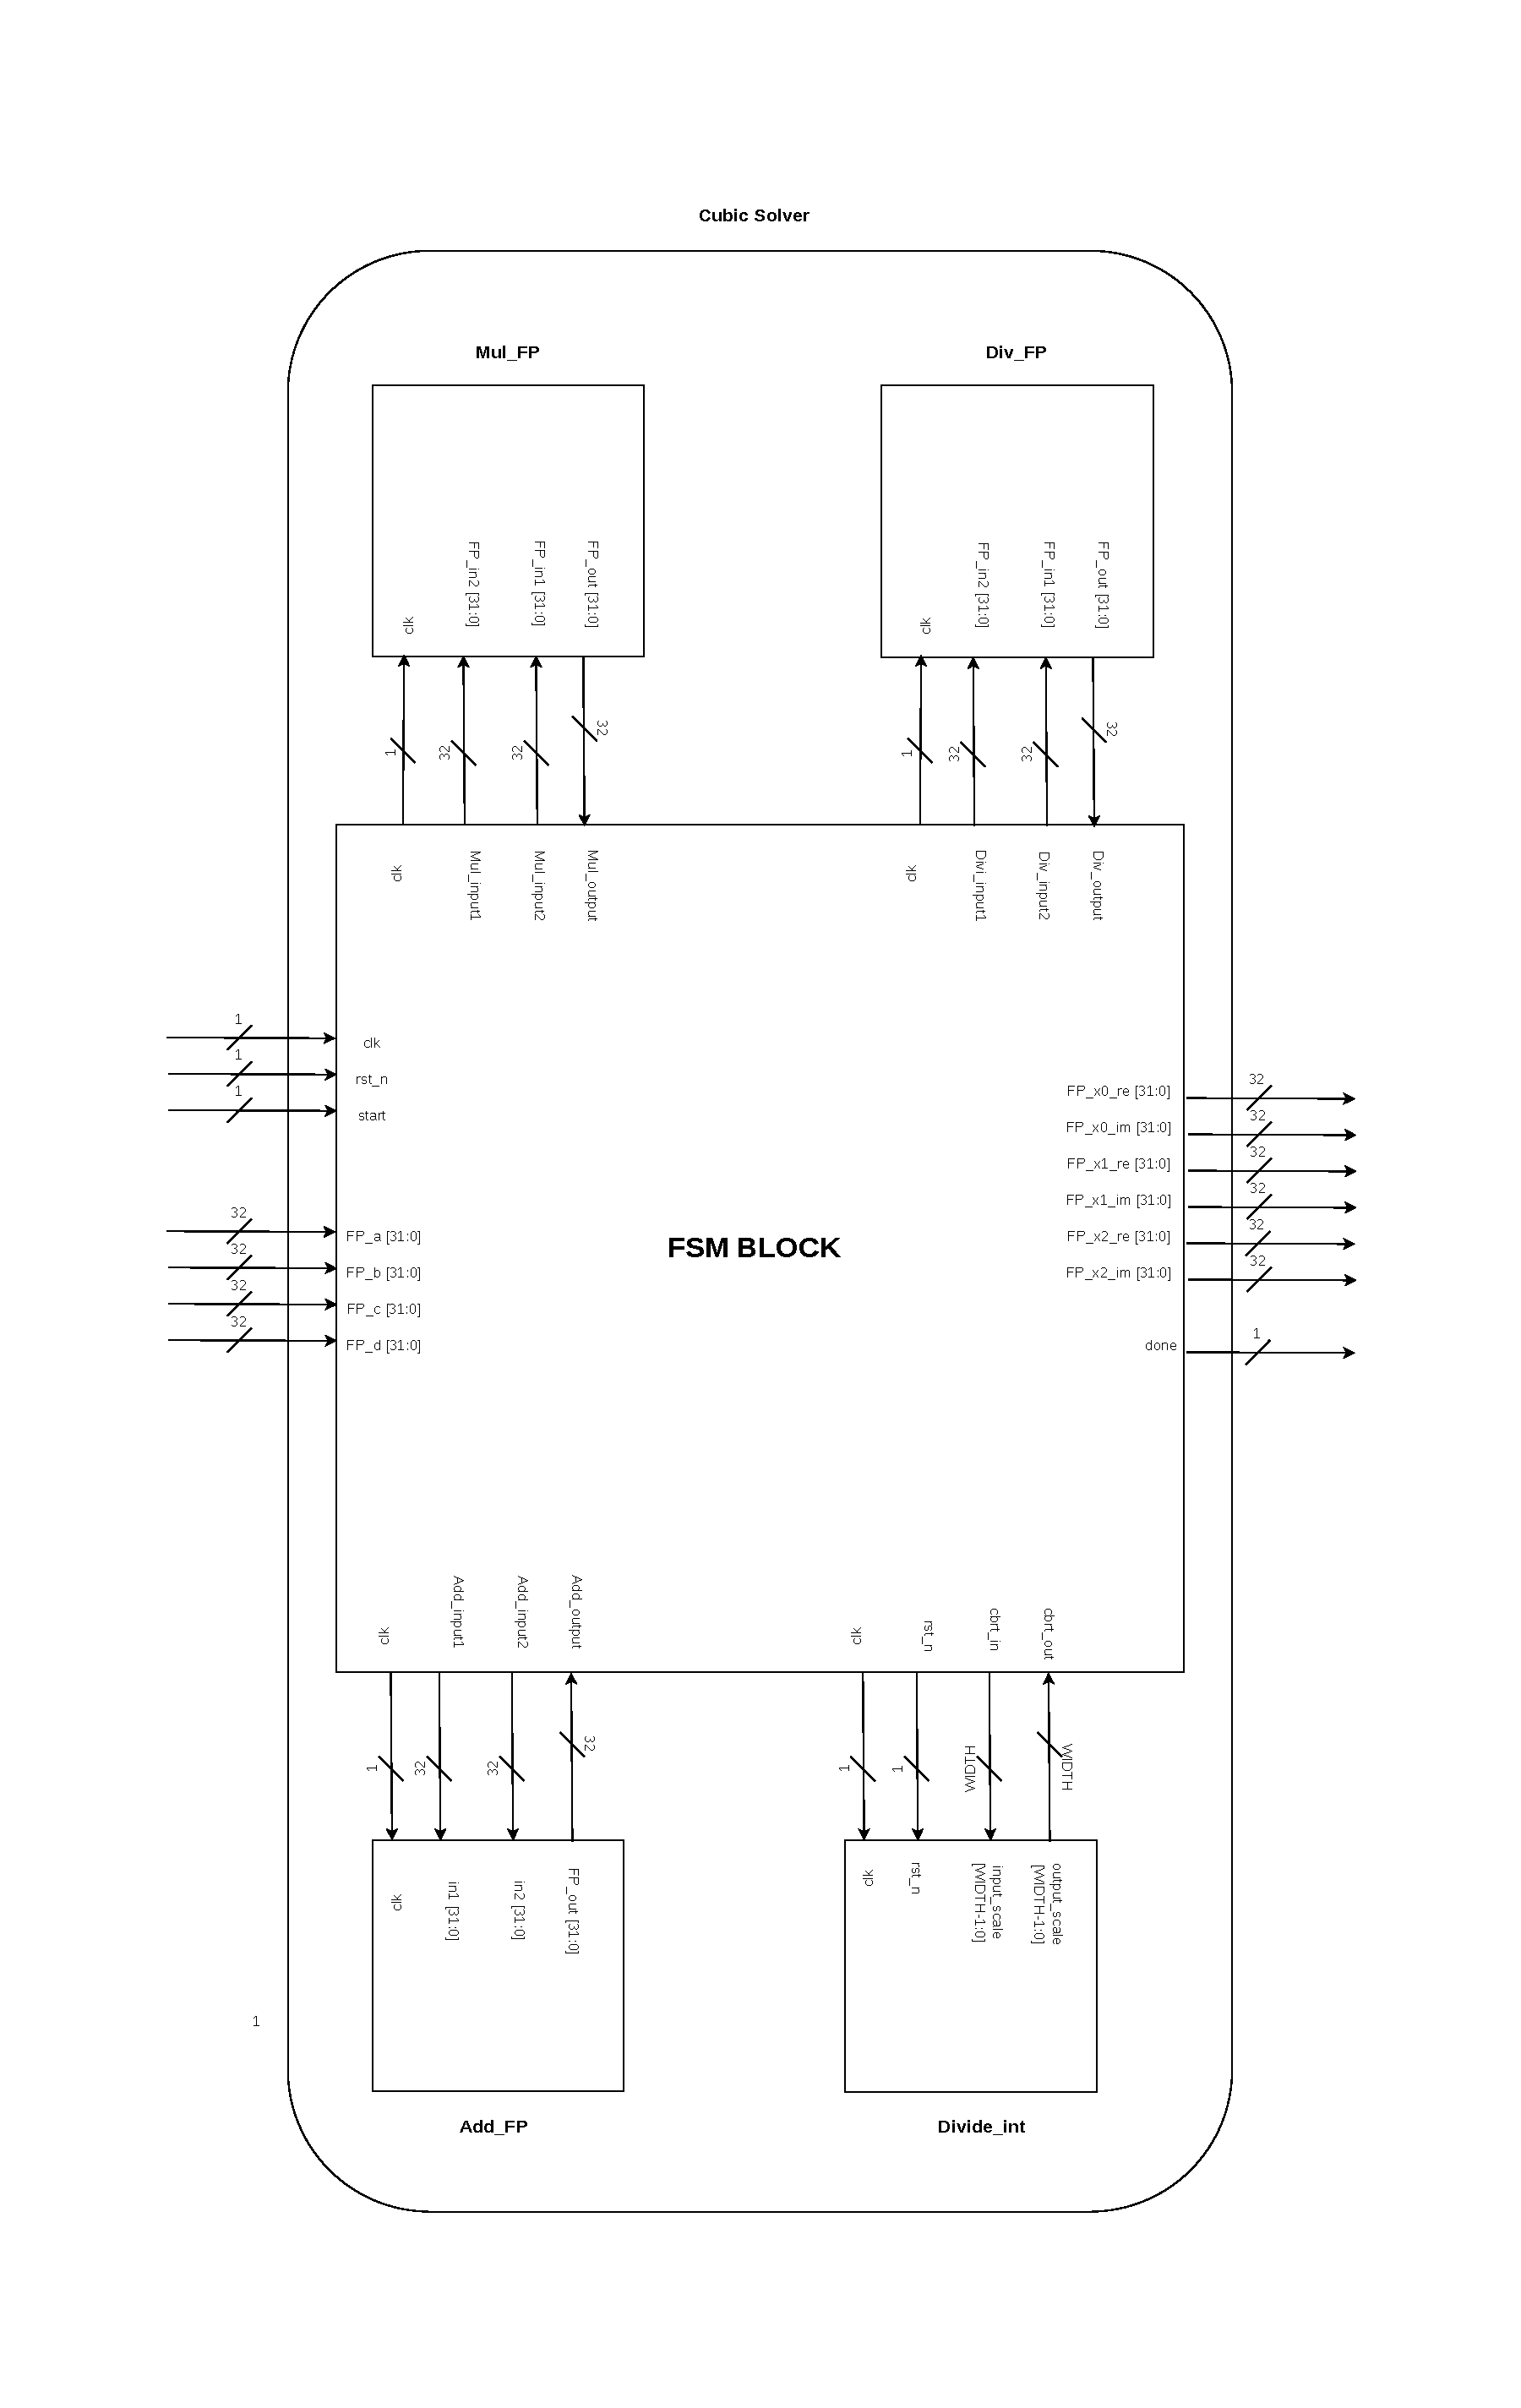
\includegraphics[width=0.70\linewidth]{graphics/Cubic_Solver.pdf}
    \caption{Internal structure of the \texttt{Cubic\_Solver} module.}
    \label{fig:cubic_solver_internal}
\end{figure}

The hardware is organized around one shared arithmetic datapath and one supervisory finite state machine. The datapath contains three floating-point operators, a small exponent-scaling helper for cube-root initialization, and a register bank for intermediate values. The controller then issues operands to the arithmetic blocks according to a cycle-by-cycle schedule encoded by \texttt{delay\_count}.

\begin{table}[H]
\centering
\caption{Main internal components of the cubic-solver architecture}
\renewcommand{\arraystretch}{1.2}
\begin{tabular}{p{3.0cm} p{2.0cm} p{1.4cm} p{8.0cm}}
\toprule
\textbf{Component} & \textbf{Signal role} & \textbf{Width} & \textbf{Description} \\
\midrule
\texttt{Add\_FP} & Add/sub datapath & 32 & Shared floating-point adder used in coefficient normalization, discriminant evaluation, Pad\'e iteration, and final root composition. \\
\texttt{Mul\_FP} & Multiply datapath & 32 & Shared floating-point multiplier used for powers, scaled terms, and complex arithmetic. \\
\texttt{Div\_FP} & Divide datapath & 32 & Shared floating-point divider used in normalization and iterative updates. \\
\texttt{Divide\_int} & Exponent helper & 8 & Approximates exponent scaling for the cube-root initial estimate. \\
\texttt{r\_temp[0:63]} & Scratch register bank & 32 & Stores partial results from pipeline outputs so later delay slots can reuse them. \\
\texttt{state}/\texttt{next\_state} & FSM controller & 4 & Controls the macro-phase of the algorithm. \\
\texttt{delay\_count} & Micro-scheduler & 7 & Aligns operator inputs with the latency of shared arithmetic units. \\
\texttt{iteration\_count} & Iteration tracker & 5 & Counts the number of Pad\'e updates performed. \\
\bottomrule
\end{tabular}
\end{table}

\subsection{Internal implementation of the arithmetic modules}

\subsubsection{\texttt{Add\_FP}}

\begin{figure}[H]
    \centering
    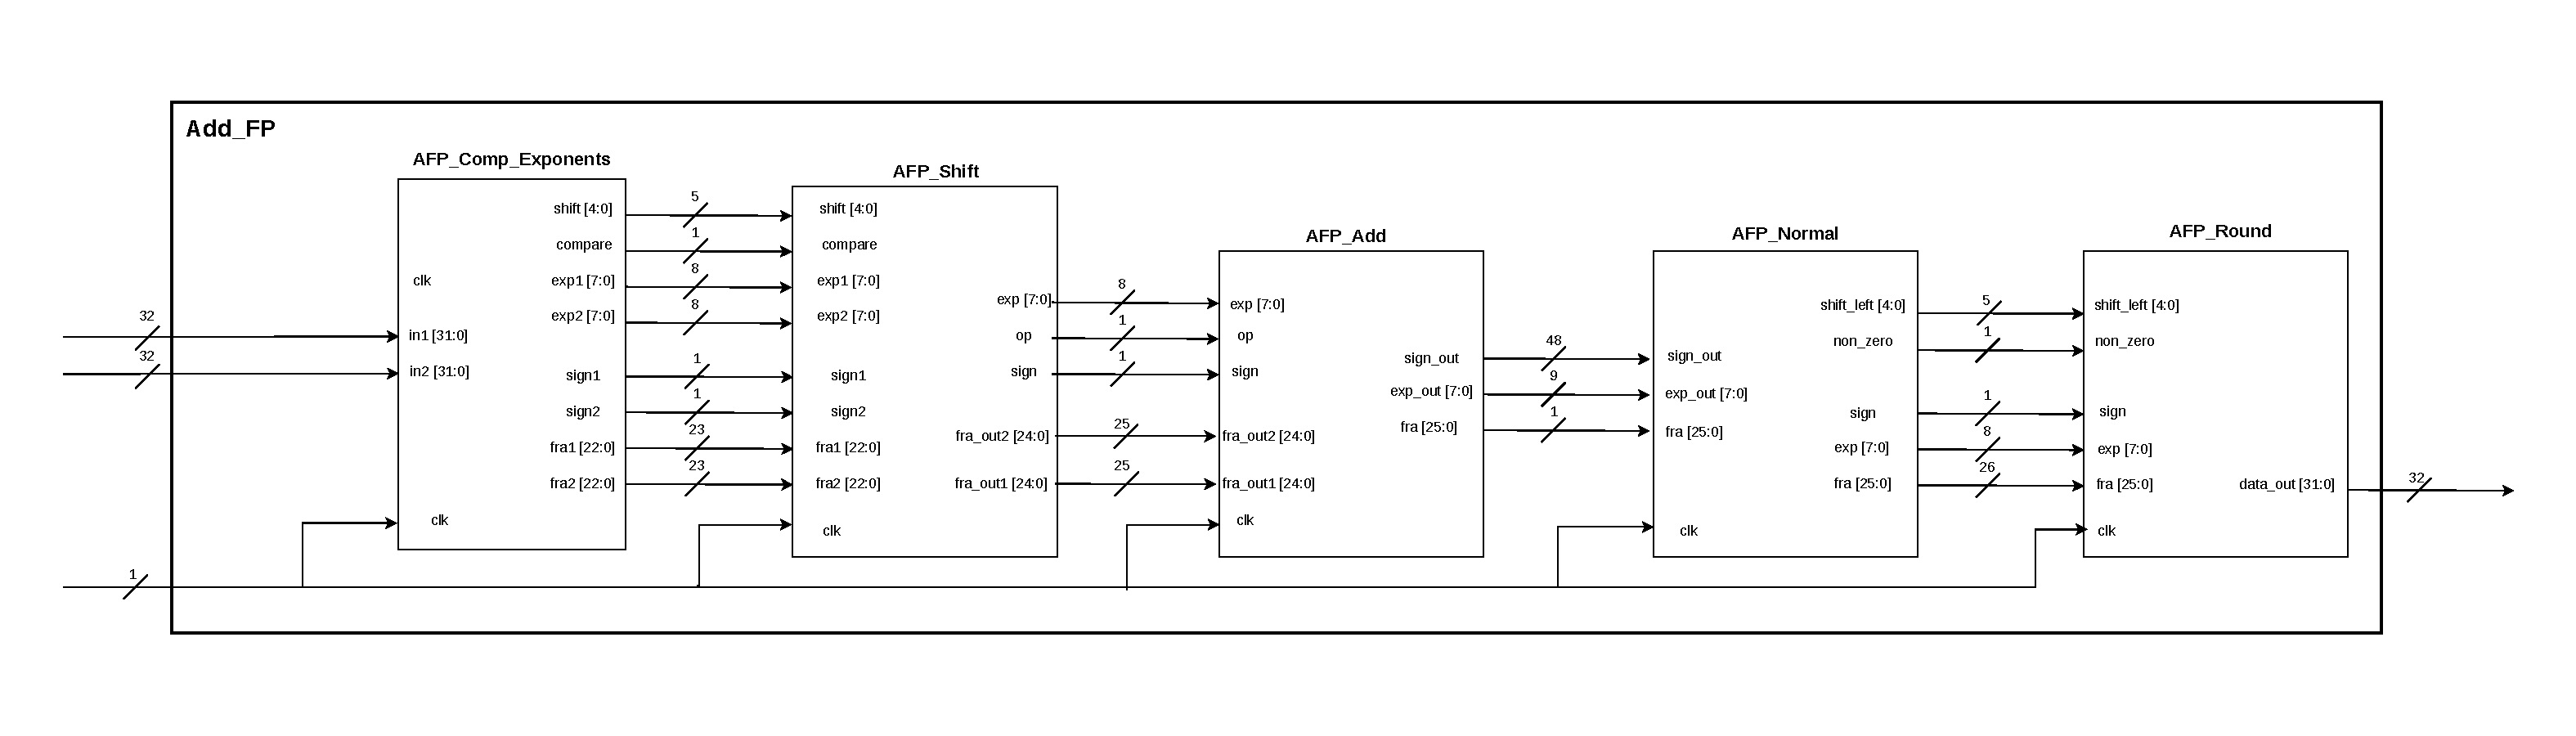
\includegraphics[width=0.95\linewidth]{graphics/Add_FP.pdf}
    \caption{Internal structure of the \texttt{Add\_FP} pipeline.}
    \label{fig:add_internal}
\end{figure}

The proposed floating-point adder is compliant with the IEEE-754 single-precision format and is implemented as a 5-stage pipeline. Instead of performing all operations in one large combinational block, the datapath is decomposed into smaller functional stages so that alignment, arithmetic, and normalization can be handled in an orderly and timing-friendly manner. The operation of each stage is summarized as follows:
\begin{itemize}
    \item \textbf{Stage 1: Exponent Comparison (\texttt{AFP\_Compare\_Exponents}).} This stage compares the exponent fields of the two operands and computes the absolute exponent difference
    \begin{equation}
        \delta = |E_A - E_B|
    \end{equation}
    to determine the alignment shift amount. At the same time, it identifies which operand has the larger exponent, preserves the sign bits, and forwards the fraction fields to the next stage.

    \item \textbf{Stage 2: Mantissa Alignment (\texttt{AFP\_Shift}).} The significand of the smaller operand is right-shifted by $\delta$ positions so that both operands share the same binary-point position. The larger operand is passed forward without loss of significance. Internally, this stage also forms the effective operation mode
    \begin{equation}
        \texttt{op} = S_A \oplus S_B
    \end{equation}
    so that the next stage knows whether the mantissas must be added or subtracted.

    \item \textbf{Stage 3: Arithmetic Operation (\texttt{AFP\_Add}).} The aligned mantissas are combined according to the effective operation sign. Functionally, this stage evaluates
    \begin{equation}
        M_{sum} = M_{large} \pm M_{shifted}
    \end{equation}
    and then converts the result back into sign-magnitude form. If the subtraction result is negative, the sign is inverted and the magnitude is stored as a positive number to simplify normalization.

    \item \textbf{Stage 4: Normalization Detection (\texttt{AFP\_Normal}).} This stage determines whether the arithmetic result is already normalized. In subtraction cases, leading zeros may appear at the MSB side of the mantissa. A priority encoder is therefore used to detect the position of the leading one and to compute the left-shift amount needed to restore the format
    \begin{equation}
        1.xxxxx
    \end{equation}
    expected by IEEE-754.

    \item \textbf{Stage 5: Normalization and Packing (\texttt{AFP\_Rounding}).} The mantissa is shifted according to the result of Stage 4, and the exponent is adjusted accordingly. If an overflow carry exists, the exponent is incremented; otherwise, it is reduced by the normalization shift amount. Finally, the result is packed back into a 32-bit IEEE-754 word.
\end{itemize}

This 5-stage organization is particularly suitable for the cubic solver because the top-level controller repeatedly issues additions such as $\Delta_0 = b^2 + c$, $\Delta = \Delta_1^2 - 4\Delta_0^3$, or the accumulation terms required by the Pad\'e iterations. A deeply regular pipeline therefore gives both structural clarity and predictable timing.

\subsubsection{\texttt{Mul\_FP}}

\begin{figure}[H]
    \centering
    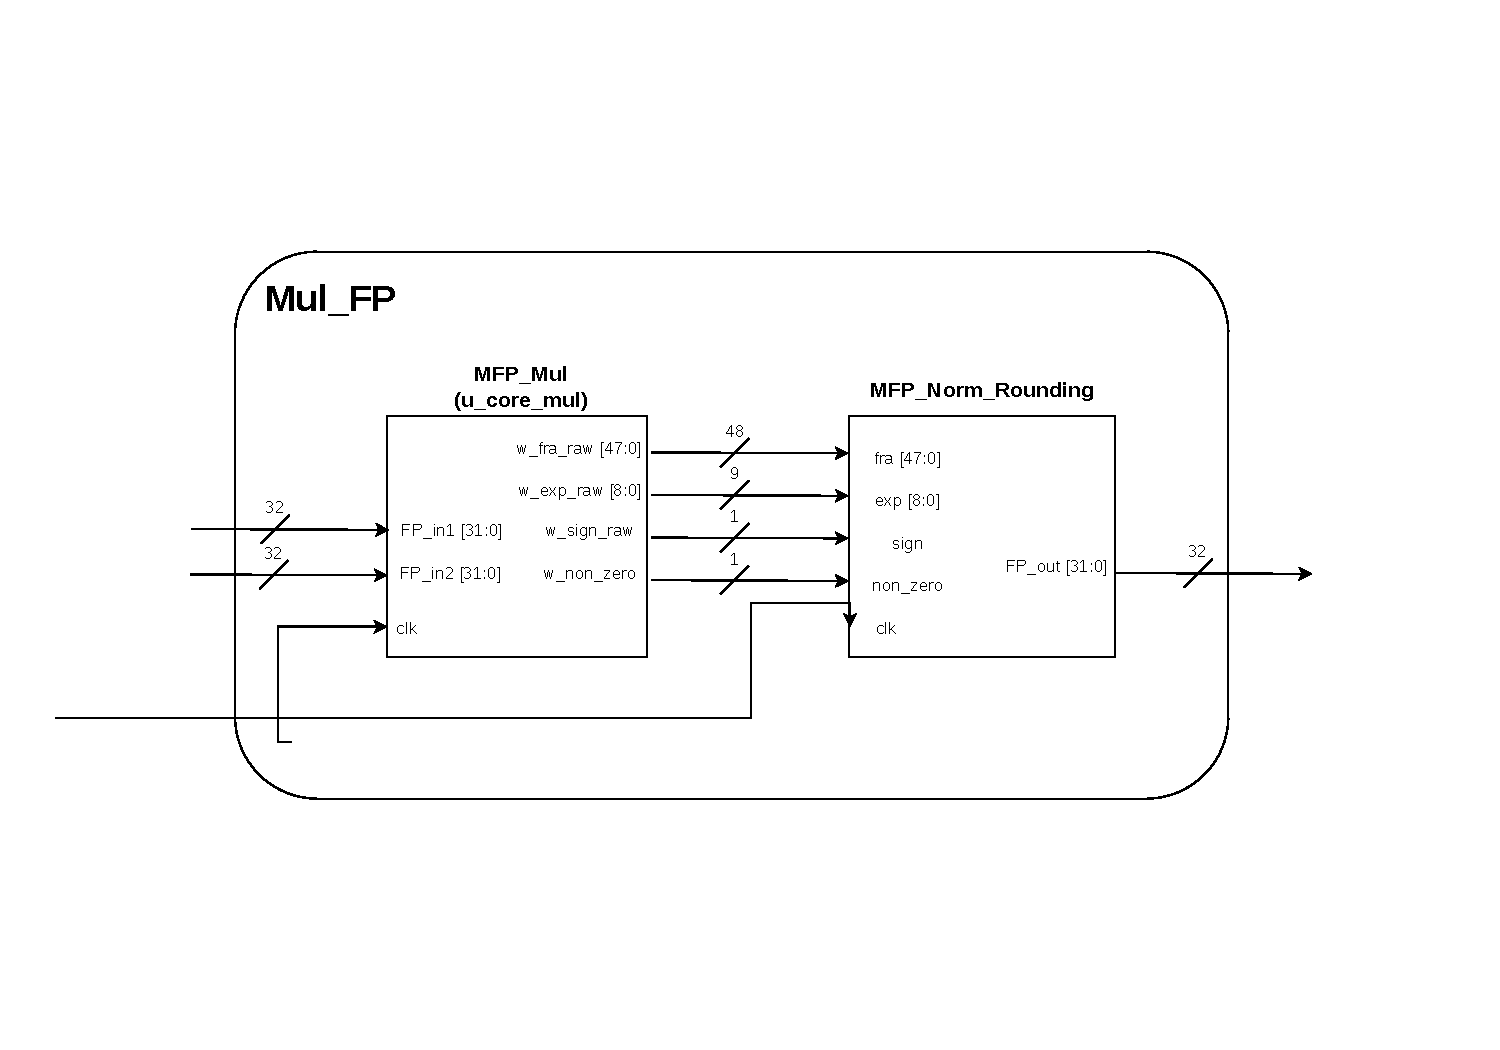
\includegraphics[width=0.92\linewidth]{graphics/Mul_FP.pdf}
    \caption{Top-level structure of the \texttt{Mul\_FP} module.}
    \label{fig:mul_internal}
\end{figure}

\begin{figure}[H]
    \centering
    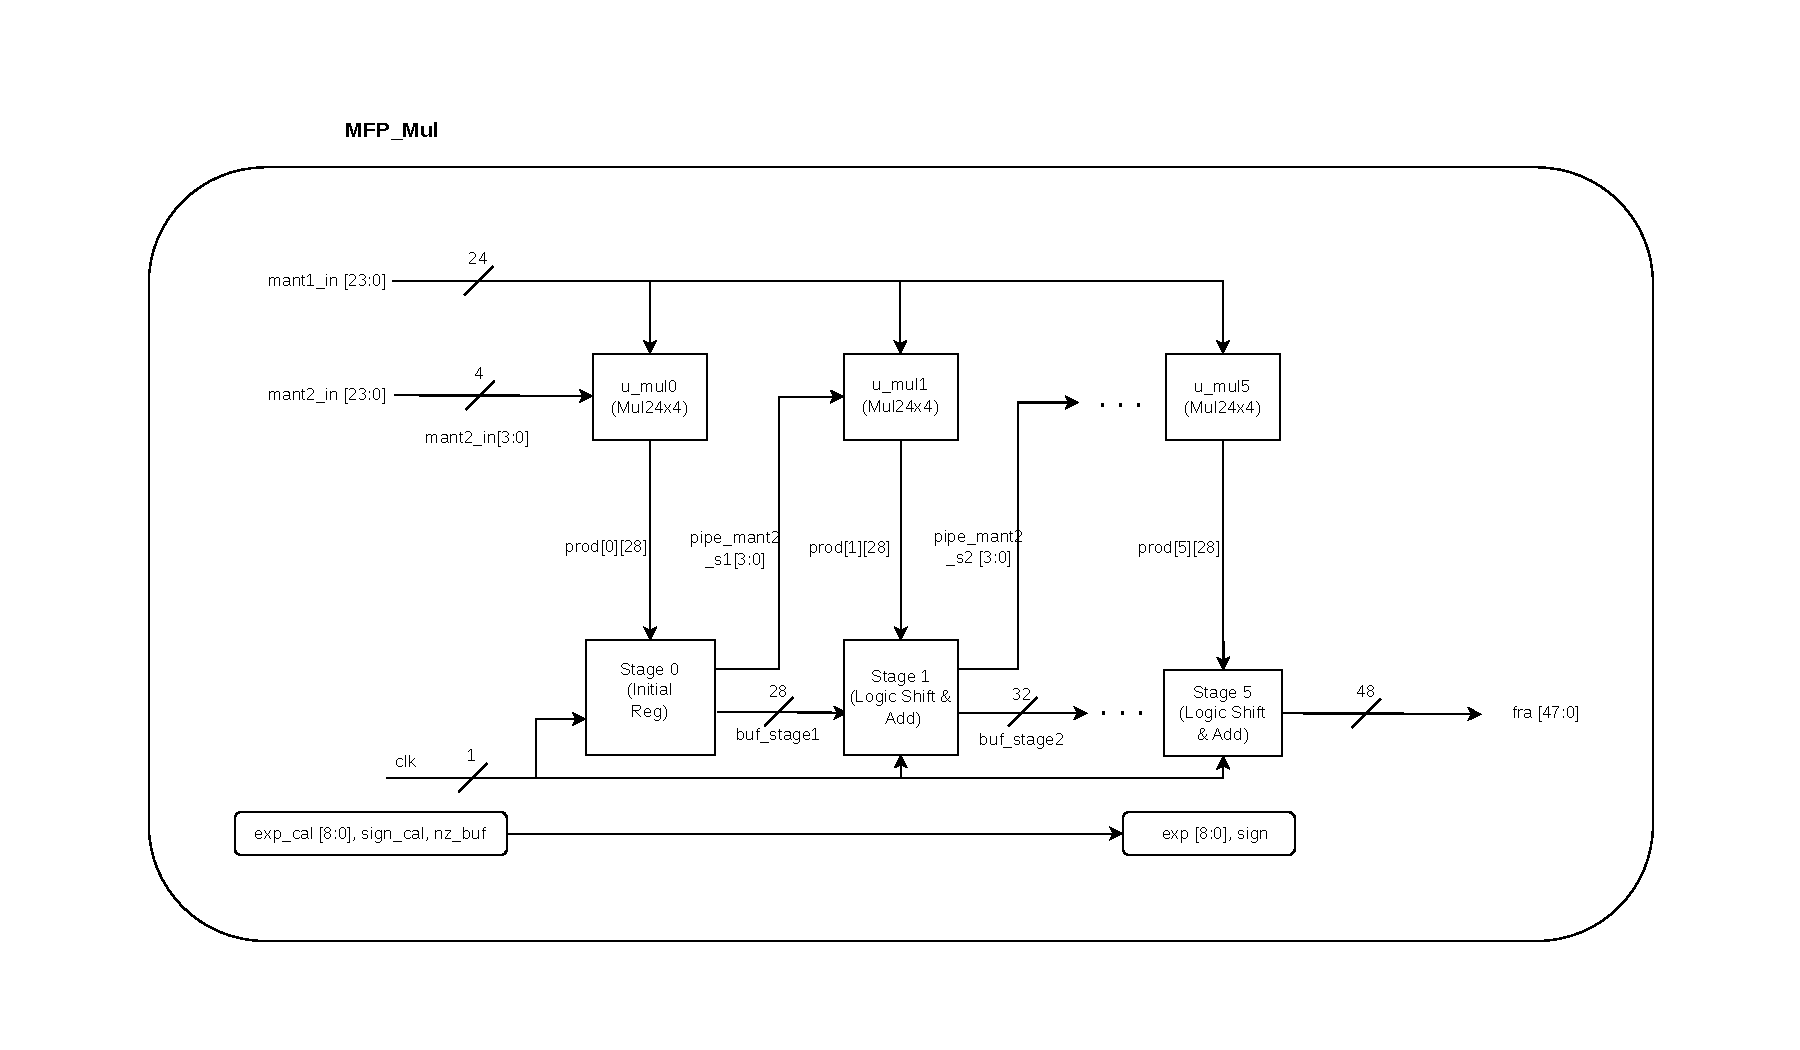
\includegraphics[width=0.92\linewidth]{graphics/MFP_Mul.pdf}
    \caption{Mantissa-multiplication core used by \texttt{Mul\_FP}.}
    \label{fig:mfp_mul_internal}
\end{figure}

To maintain high throughput and keep the critical path short, the multiplier avoids a single-cycle 24$\times$24-bit mantissa multiplication. Instead, the architecture uses a staged 4-bit nibble-decomposition strategy. The complete \texttt{Mul\_FP} block can therefore be understood as a 7-stage pipeline: 6 stages for mantissa partial-product accumulation and 1 stage for normalization and final packing.

\paragraph{Pre-processing}
Before mantissa multiplication begins, the two FP32 operands are decomposed into sign, exponent, and fraction fields. The hidden bit is appended to both fractions to form
\begin{equation}
M_A = \{1, frac_A\}, \qquad M_B = \{1, frac_B\}
\end{equation}
The tentative exponent is computed as
\begin{equation}
E_{raw} = E_A + E_B - 127
\end{equation}
and the output sign is obtained by XOR:
\begin{equation}
S_{out} = S_A \oplus S_B
\end{equation}

\paragraph{Partial Product Accumulation (Stages 1--6)}
The core multiplication logic decomposes the 24-bit multiplier mantissa into six 4-bit nibbles. In each stage $i$ ($i = 0 \dots 5$), one \texttt{Mul24x4} block computes a 24$\times$4-bit partial product, and this new contribution is accumulated with the previously stored partial sum. Conceptually, the recurrence can be interpreted as
\begin{equation}
P_i = (P_{i-1} \ll 4) + \left(M_A \times M_B[4i+3:4i]\right)
\end{equation}
where each nibble contributes one radix-$2^4$ digit of the final mantissa product.

The stage-by-stage meaning is:
\begin{itemize}
    \item \textbf{Stage 1:} use \texttt{mant2\_in[3:0]} and store the first partial product in \texttt{buf\_stage1}.
    \item \textbf{Stage 2:} use the next nibble and accumulate into \texttt{buf\_stage2}.
    \item \textbf{Stage 3:} accumulate the contribution of bits \texttt{[11:8]} into \texttt{buf\_stage3}.
    \item \textbf{Stage 4:} accumulate the contribution of bits \texttt{[15:12]} into \texttt{buf\_stage4}.
    \item \textbf{Stage 5:} accumulate the contribution of bits \texttt{[19:16]} into \texttt{buf\_stage5}.
    \item \textbf{Stage 6:} accumulate the final nibble \texttt{[23:20]} and generate the full 48-bit raw product \texttt{fra}.
\end{itemize}

This nibble-based organization ensures that the combinational depth of each stage remains shallow. Instead of building a large and timing-expensive multiplier tree, the architecture spreads the work across several short pipeline stages.

\paragraph{Normalization and Final Packaging (Final Stage)}
Once the raw 48-bit product has been formed, the block \texttt{MFP\_Norm\_Rounding} performs IEEE-754 post-processing:
\begin{itemize}
    \item \textbf{Normalization:} The block checks whether the most significant bit of the 48-bit raw product is already in normalized position. Depending on that condition, it selects either \texttt{fra[46:23]} or \texttt{fra[45:22]} as the normalized mantissa slice and updates the exponent.
    \item \textbf{Rounding:} The least significant dropped bit is used to realize round-to-nearest behavior before the final 23-bit fraction is stored.
    \item \textbf{Packing:} The sign, normalized exponent, and rounded mantissa are concatenated into the final FP32 result.
\end{itemize}

This architecture is efficient for the current application because the solver repeatedly needs products such as $\hat{b}^2$, $\hat{b}^3$, $\Delta_0^3$, $\Delta_1^2$, and the large set of cross-products required by the complex cube-root branch.

\subsubsection{\texttt{Div\_FP}}

\begin{figure}[H]
    \centering
    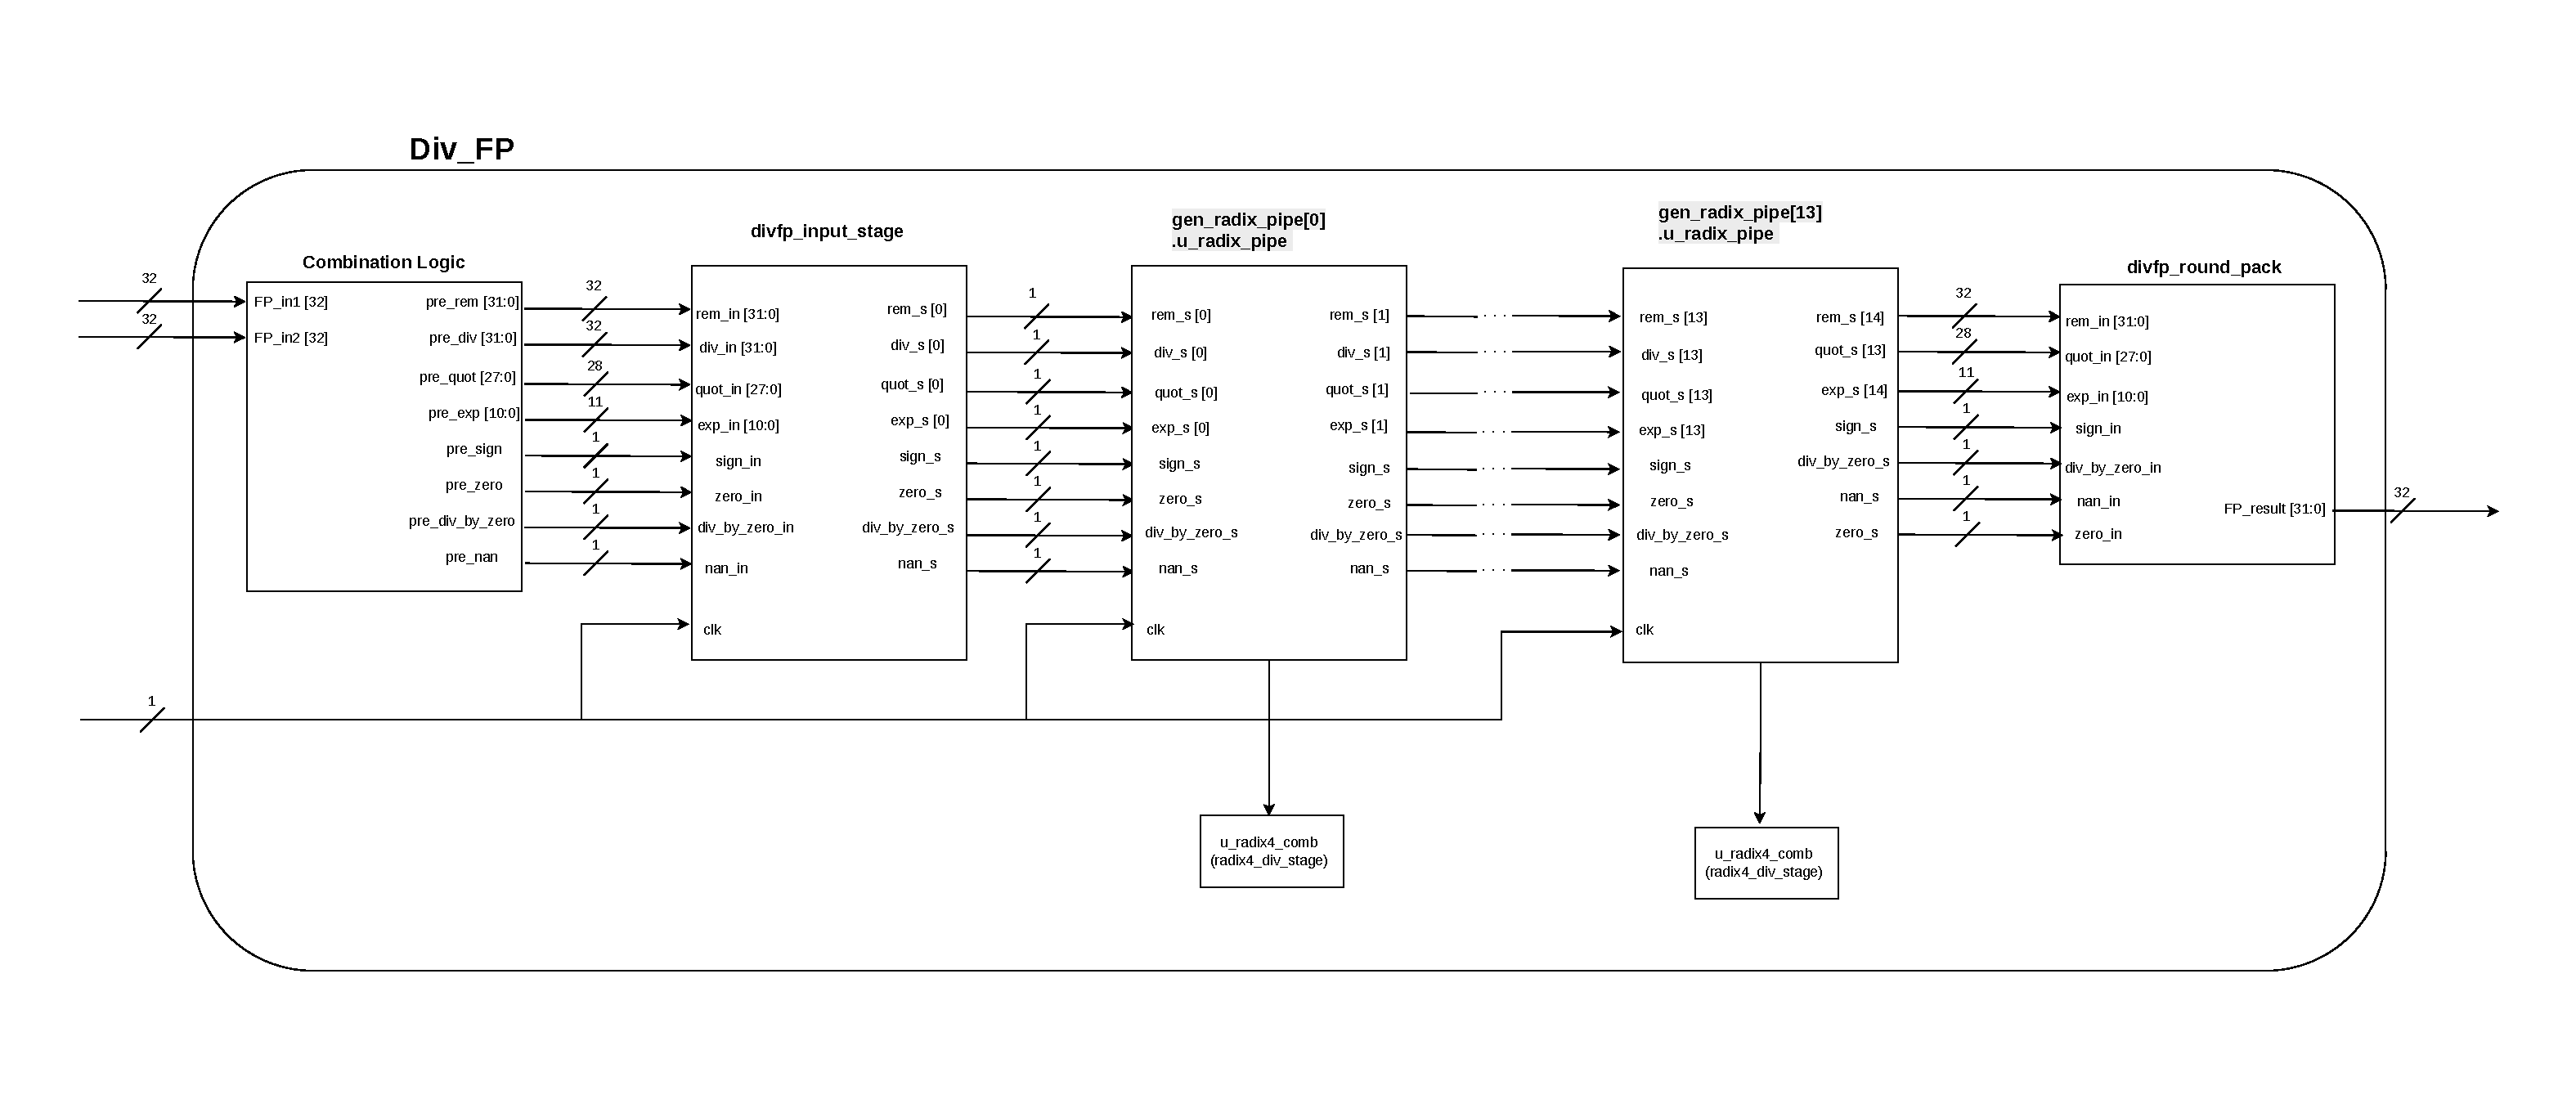
\includegraphics[width=0.95\linewidth]{graphics/Div_FP.pdf}
    \caption{Internal structure of the \texttt{Div\_FP} module.}
    \label{fig:div_internal}
\end{figure}

The division unit is designed as a radix-4 pipelined floating-point divider. Similar to the multiplier, the goal is not minimum latency in a single cycle, but rather a regular multi-stage implementation with deterministic throughput and timing behavior. The full \texttt{Div\_FP} datapath can be interpreted as a 16-cycle pipeline: 1 input stage, 14 radix-4 quotient-generation stages, and 1 output register stage.

\paragraph{Stage 1: Pre-processing and operand standardization}
The first step extracts sign, exponent, and fraction fields from the two FP32 operands. The divider then classifies special cases:
\begin{itemize}
    \item zero numerator
    \item zero denominator
    \item NaN / special exponent cases
\end{itemize}
The output sign is computed as
\begin{equation}
S_{out} = S_A \oplus S_B
\end{equation}
and the initial exponent is formed from the exponent difference between dividend and divisor. To ensure that the mantissa quotient starts in normalized range, the design compares the two mantissas:
\begin{itemize}
    \item if $M_A < M_B$, the dividend mantissa is left-shifted and the exponent is biased by 126
    \item otherwise, the mantissa is used directly and the exponent is biased by 127
\end{itemize}
This step creates the initial remainder \texttt{pre\_rem}, divisor \texttt{pre\_div}, quotient register \texttt{pre\_quot}, and exponent \texttt{pre\_exp}.

\paragraph{Stage 2: Input pipeline register}
The standardized division operands are stored in \texttt{divfp\_input\_stage}. This stage isolates the combinational preprocessing logic from the iterative radix-4 quotient datapath and guarantees synchronous propagation of the control metadata such as sign, zero flag, division-by-zero flag, and NaN flag.

\paragraph{Stages 3--16: Radix-4 quotient generation}
The main body of the divider consists of fourteen identical registered radix-4 stages. In each stage, the combinational block \texttt{radix4\_div\_stage} performs the following operations:
\begin{itemize}
    \item shift the current remainder left by 2 bits
    \item compare the shifted remainder with $2D$ and $D$
    \item subtract the largest possible multiple without making the remainder negative
    \item emit one quotient digit \texttt{q\_digit} in radix-4, equivalent to two binary quotient bits
\end{itemize}

If the stage remainder is denoted by $R_i$ and the divisor by $D$, then each stage evaluates
\begin{equation}
R_i' = 4R_i
\end{equation}
and chooses a quotient digit $q_i \in \{0,1,2,3\}$ such that
\begin{equation}
R_{i+1} = 4R_i - q_iD
\end{equation}
remains non-negative. The digit is appended into the running quotient register. Since each stage contributes two quotient bits, fourteen stages are sufficient to build a 28-bit quotient representation.

\paragraph{Final stage: Rounding and IEEE-754 packaging}
After the last radix-4 stage, the block \texttt{divfp\_round\_pack} reconstructs the floating-point result:
\begin{itemize}
    \item the quotient bits are converted into a normalized mantissa candidate
    \item guard, round, and sticky information are used to implement round-to-nearest
    \item the exponent is corrected if the rounding operation produces mantissa overflow
    \item special conditions such as NaN, division by zero, overflow, and underflow are handled before final packing
\end{itemize}
The result is then registered once more into \texttt{FP\_out}, completing the division pipeline.

The fixed latency of this divider is particularly important for the cubic solver. Since the top-level design contains only one instance of \texttt{Div\_FP}, the FSM must know exactly when a valid quotient becomes available. The regular 16-cycle structure is therefore a major advantage for state scheduling.

\subsection{Finite state machine}

\begin{figure}[H]
    \centering
    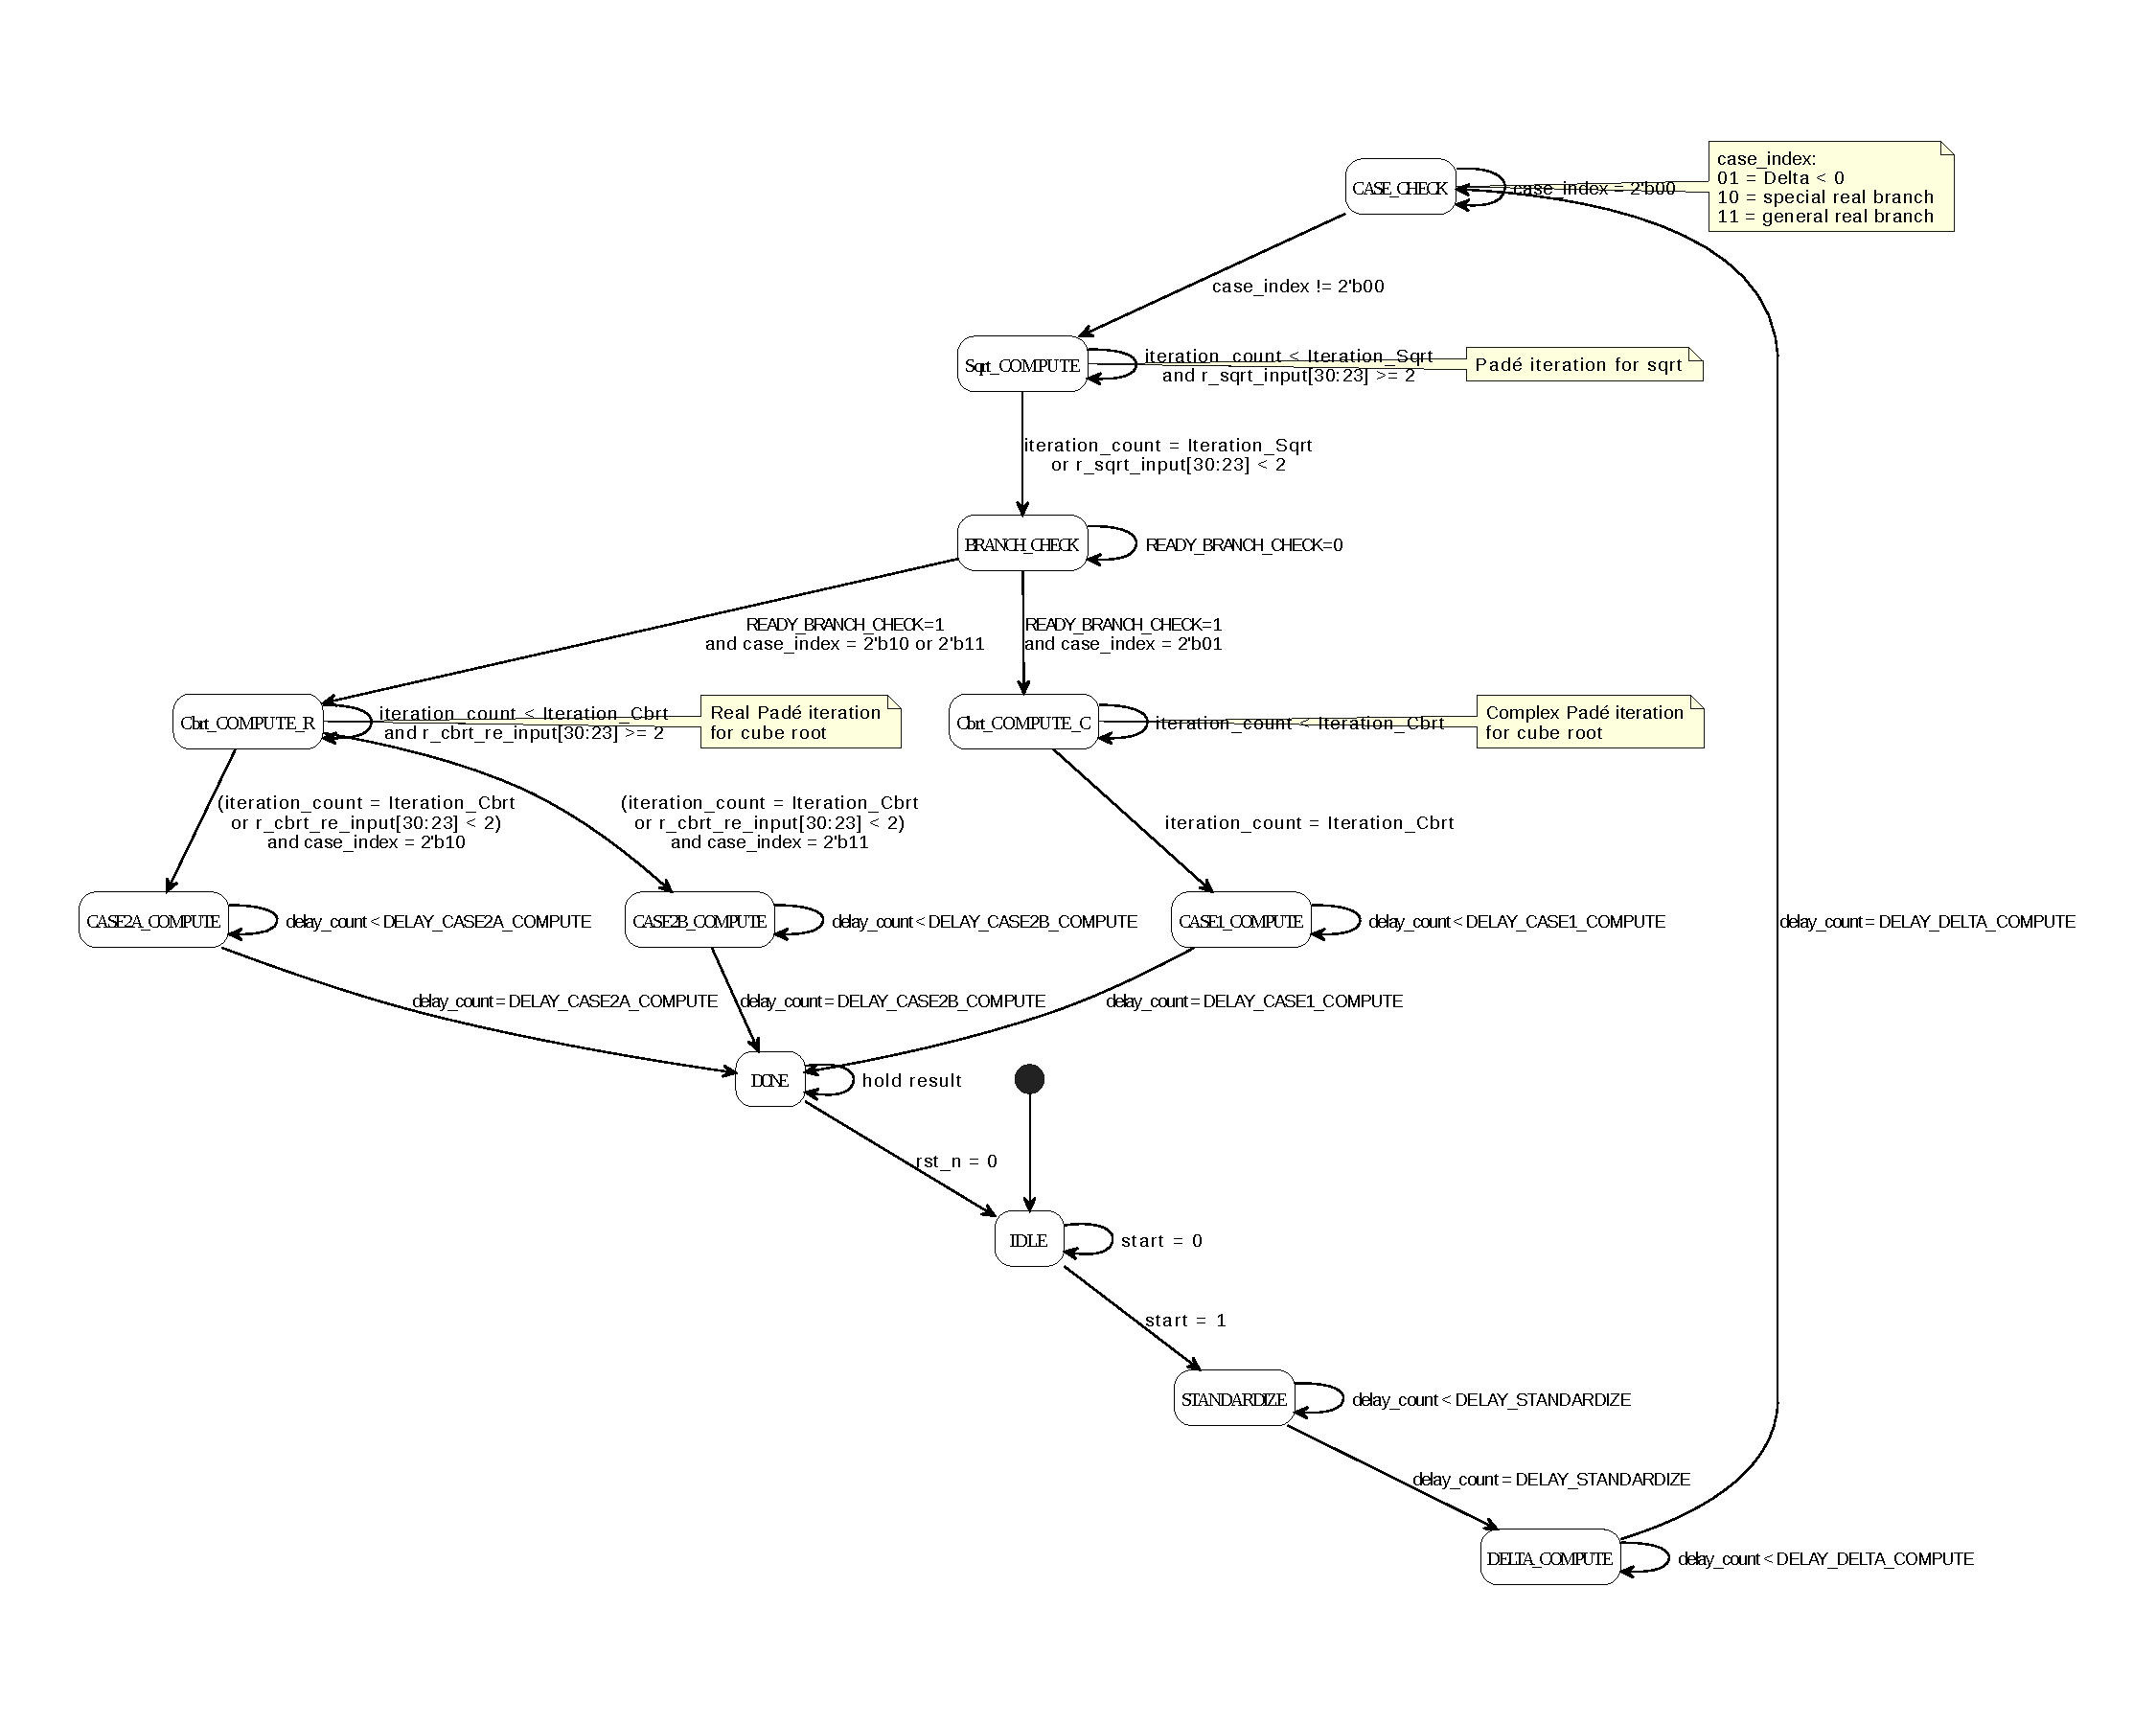
\includegraphics[width=0.95\linewidth]{graphics/FSM.pdf}
    \caption{Finite state machine of the \texttt{Cubic\_Solver} module.}
    \label{fig:cubic_solver_fsm}
\end{figure}

\subsubsection{State summary}

\begin{table}[H]
\centering
\caption{State encoding and role of the main solver FSM}
\renewcommand{\arraystretch}{1.2}
\begin{tabular}{lll p{7.8cm}}
\toprule
\textbf{State} & \textbf{Code} & \textbf{Phase} & \textbf{Main responsibility} \\
\midrule
\texttt{IDLE} & \texttt{4'b0000} & Wait & Wait for \texttt{start}, capture input coefficients, and initialize counters. \\
\texttt{STANDARDIZE} & \texttt{4'b0001} & Pre-process & Compute normalized coefficients by dividing $b$, $c$, and $d$ by $-3a$. \\
\texttt{DELTA\_COMPUTE} & \texttt{4'b0010} & Invariant generation & Compute $\Delta_0$, $\Delta_1$, and $\Delta$. \\
\texttt{CASE\_CHECK} & \texttt{4'b0011} & Branch selection & Encode the solving branch into \texttt{case\_index} and initialize the square-root stage. \\
\texttt{Sqrt\_COMPUTE} & \texttt{4'b0100} & Iteration & Run Pad\'e square-root iteration. \\
\texttt{BRANCH\_CHECK} & \texttt{4'b0101} & Dispatch & Prepare cube-root inputs and initial estimates for the chosen branch. \\
\texttt{Cbrt\_COMPUTE\_R} & \texttt{4'b0110} & Iteration & Run the real cube-root Pad\'e iteration. \\
\texttt{Cbrt\_COMPUTE\_C} & \texttt{4'b0111} & Iteration & Run the complex cube-root Pad\'e iteration. \\
\texttt{CASE1\_COMPUTE} & \texttt{4'b1000} & Output synthesis & Generate roots for the negative-discriminant branch. \\
\texttt{CASE2A\_COMPUTE} & \texttt{4'b1001} & Output synthesis & Generate roots for the simplified real branch. \\
\texttt{CASE2B\_COMPUTE} & \texttt{4'b1010} & Output synthesis & Generate roots for the general real branch. \\
\texttt{DONE} & \texttt{4'b1011} & Handshake & Assert \texttt{done} and hold valid outputs. \\
\bottomrule
\end{tabular}
\end{table}

\subsubsection{Detailed analysis of each state}

\paragraph{1. \texttt{IDLE}}
This is the reset and wait state. The solver stores the external coefficients into \texttt{r\_a}, \texttt{r\_b}, \texttt{r\_c}, and \texttt{r\_d}, clears \texttt{delay\_count}, \texttt{iteration\_count}, and \texttt{case\_index}, and waits until \texttt{start = 1}. No arithmetic operator is actively driven in this state.

\paragraph{2. \texttt{STANDARDIZE}}
The controller converts the equation to the normalized form used by the mathematical model. At the beginning of the state, the solver computes $3a$ by adding \texttt{r\_a} and \texttt{2a}, where \texttt{2a} is produced by exponent shifting. The resulting term is negated and used as the divisor for three sequential divisions:
\begin{itemize}
    \item \texttt{r\_b / (-3a)}
    \item \texttt{r\_c / (-3a)}
    \item \texttt{r\_d / (-3a)}
\end{itemize}
The outputs are written back into the working coefficient registers. This state therefore converts the external polynomial description into the internal algebraic form used by all following states.

\paragraph{3. \texttt{DELTA\_COMPUTE}}
This state computes the invariants $\Delta_0$, $\Delta_1$, and $\Delta$ by a carefully scheduled sequence of multiply-add operations:
\begin{itemize}
    \item \textbf{Early slots}: compute $\hat{b}^2$ and $\hat{b}\hat{c}$.
    \item \textbf{Middle slots}: form $\Delta_0 = \hat{b}^2 + \hat{c}$ and $2\hat{b}^3 + 3\hat{b}\hat{c} + 3\hat{d}$.
    \item \textbf{Late slots}: form $\Delta_1^2$, $4\Delta_0^3$, and finally $\Delta = \Delta_1^2 - 4\Delta_0^3$.
\end{itemize}
The state stores partial results in \texttt{r\_temp[0]} and the final invariant values in \texttt{r\_delta\_0}, \texttt{r\_delta\_1}, \texttt{r\_delta\_0\_Compare}, and \texttt{r\_delta}.

\paragraph{4. \texttt{CASE\_CHECK}}
Once the discriminant terms are available, the solver decides which branch of the cubic formula must be executed next. This state is therefore the main decision point of the entire algorithm. Conceptually, the FSM divides the problem into three cases:
\begin{itemize}
    \item \textbf{Case 1 -- complex branch} (\texttt{case\_index = 2'b01}): selected when $\Delta < 0$. In this case, the hardware must interpret $\sqrt{\Delta}$ as a purely imaginary quantity and later perform a complex-valued cube-root iteration.
    \item \textbf{Case 2A -- simplified real branch} (\texttt{case\_index = 2'b10}): selected when the special repeated-root condition is detected. The subsequent cube-root stage only needs a real-valued operand derived from $\Delta_1$.
    \item \textbf{Case 2B -- general real branch} (\texttt{case\_index = 2'b11}): selected for all remaining cases. The solver must later compute both $C$ and $\Delta_0/C$ to reconstruct the final roots.
\end{itemize}

Besides selecting the branch, this state also prepares the square-root phase:
\begin{itemize}
    \item \texttt{r\_sqrt\_input} is loaded with either $\Delta$ or $-\Delta$, depending on whether the square root must be treated as real or imaginary.
    \item \texttt{r\_sqrt\_output} is initialized with \texttt{sqrt\_output\_init}, which is an exponent-based first estimate derived from the operand magnitude.
    \item \texttt{iteration\_count} is cleared so that the Pad\'e loop starts from its first iteration.
\end{itemize}
Functionally, \texttt{CASE\_CHECK} is the bridge between discriminant evaluation and the branch-specific numerical refinement process.

\paragraph{5. \texttt{Sqrt\_COMPUTE}}
This state implements the Pad\'e update for square root:
\begin{equation}
P_{n+1} = P_n \cdot \frac{P_n^2 + 3S}{3P_n^2 + S}
\end{equation}
Before the iterative loop starts, the initial estimate $P_0$ is not chosen arbitrarily. The RTL forms it by manipulating the exponent of the operand:
\begin{equation}
\texttt{sqrt\_output\_exp = ((exp(S) + 127) >> 1)}
\end{equation}
and then reconstructs a provisional FP32 value with the same mantissa field:
\begin{equation}
\texttt{sqrt\_output\_init = \{0, sqrt\_output\_exp, mantissa(S)\}}
\end{equation}
This is an exponent-based magnitude approximation to $\sqrt{S}$, and it provides a much better starting point than a constant seed.

The controller dispatches arithmetic operations over multiple delay slots:
\begin{itemize}
    \item compute $P_n^2$,
    \item compute $3S$,
    \item form $P_n^2 + 3S$ and $3P_n^2 + S$,
    \item divide the two terms after multiplying the numerator by $P_n$.
\end{itemize}
The new approximation is stored back into \texttt{r\_sqrt\_output}. The state loops until \texttt{iteration\_count} reaches \texttt{Iteration\_Sqrt} or the operand is sufficiently small.

\paragraph{6. \texttt{BRANCH\_CHECK}}
This state specializes the next phase according to \texttt{case\_index}:
\begin{itemize}
    \item For the complex branch, it forms the real and imaginary parts of $(\Delta_1 + \sqrt{\Delta})/2$ by halving \texttt{r\_delta\_1} and \texttt{r\_sqrt\_output} through exponent adjustment. The state then compares both exponents and selects the larger one as \texttt{exponent\_max} so that the complex cube-root seed has a safe magnitude.
    \item For the simplified real branch, it uses $\Delta_1$ directly as cube-root input and initializes the imaginary path to zero.
    \item For the general real branch, it first adds $\Delta_1$ and $\sqrt{\Delta}$, then divides by two to form the real cube-root input.
\end{itemize}
In all three branches, the cube-root estimate is initialized through exponent scaling rather than through a fixed numerical constant. The helper block \texttt{Divide\_int} approximates
\begin{equation}
E_{\sqrt[3]{S}} \approx 127 + \frac{E_S - 127}{3}
\end{equation}
so that the FSM can build the first cube-root estimate directly from the FP32 exponent field. The flag \texttt{READY\_BRANCH\_CHECK} is asserted when both the branch-specific operand and the corresponding initial estimate are ready, allowing the FSM to enter the correct cube-root state.

\paragraph{7. \texttt{Cbrt\_COMPUTE\_R}}
This state evaluates the real Pad\'e cube-root update
\begin{equation}
P_{n+1} = P_n \cdot \frac{P_n^3 + 2S}{2P_n^3 + S}
\end{equation}
The initial estimate $P_0$ used in this state is generated before entry by exponent scaling, not by iterative search. This means the real cube-root iteration starts from a value that already has approximately the correct order of magnitude.

The controller schedules:
\begin{itemize}
    \item $P_n^2$ and $P_n^3$,
    \item $2S$ and $2P_n^3$,
    \item the numerator and denominator sums,
    \item the final division that yields the next approximation.
\end{itemize}
At the end of the iteration budget, the result is written to \texttt{r\_C\_re} while \texttt{r\_C\_im} remains zero.

\paragraph{8. \texttt{Cbrt\_COMPUTE\_C}}
This is the most arithmetic-intensive state because it performs Pad\'e cube-root iteration on a complex operand. The state must evaluate both the numerator $P^4 + 2SP$ and the denominator $2P^3 + S$, then perform a complex division:
\begin{equation}
\frac{n_r + jn_i}{d_r + jd_i}
=
\frac{(n_rd_r + n_id_i) + j(n_id_r - n_rd_i)}{d_r^2 + d_i^2}
\end{equation}
To support this process, the controller uses a large subset of \texttt{r\_temp[]} to store partial real and imaginary products such as:
\begin{itemize}
    \item real and imaginary parts of $P^2$,
    \item real and imaginary parts of $SP$,
    \item real and imaginary parts of $P^3$ and $P^4$,
    \item the numerator and denominator of the final complex quotient.
\end{itemize}
The initial complex estimate is also generated by exponent logic. Instead of deriving separate analytical seeds for the real and imaginary parts, the hardware uses the larger exponent between both components as a conservative magnitude reference, then reconstructs FP32 seed values for \texttt{r\_cbrt\_re\_output} and \texttt{r\_cbrt\_im\_output}. This state demonstrates the main architectural idea of the project: even complex-valued iterations are realized by scheduling a small number of shared scalar FP32 arithmetic blocks.

\paragraph{9. \texttt{CASE1\_COMPUTE}}
This state generates three roots for the negative-discriminant branch. Since $C$ is complex, the solver combines \texttt{r\_C\_re}, \texttt{r\_C\_im}, and the constants $\varepsilon$ and $\varepsilon^2$ to produce
\begin{equation}
x_k = \hat{b} + \varepsilon^k C + \varepsilon^{2k}\overline{C}
\end{equation}
The outputs are written progressively into \texttt{FP\_x0\_*}, \texttt{FP\_x1\_*}, and \texttt{FP\_x2\_*} over several delay slots.

\paragraph{10. \texttt{CASE2A\_COMPUTE}}
This state handles the simplified real branch. Only one real value $C$ is needed, so the solver forms
\begin{equation}
x_k = \hat{b} + \varepsilon^k C
\end{equation}
The first root remains purely real, while the second and third roots are produced as a conjugate pair by multiplying $C$ with the real and imaginary parts of $\varepsilon$.

\paragraph{11. \texttt{CASE2B\_COMPUTE}}
This state handles the general real branch, which requires both $C$ and $\Delta_0/C$. The controller first launches the division \texttt{r\_delta\_0 / r\_C\_re}, then combines the quotient with the $\varepsilon$-scaled copies of $C$ to form:
\begin{equation}
x_k = \hat{b} + \varepsilon^k C + \varepsilon^{2k}\frac{\Delta_0}{C}
\end{equation}
Compared with \texttt{CASE2A\_COMPUTE}, this state is longer because it must wait for the divider output before the final root-reconstruction steps can be completed.

\paragraph{12. \texttt{DONE}}
The state asserts \texttt{done = 1} and holds all output roots stable. This allows the external environment to sample the results without ambiguity.

\subsection{The general operational principle of each state}

From an implementation point of view, the most important characteristic of this design is the tight coupling between FSM state and datapath issue pattern:
\begin{itemize}
    \item \textbf{State selection} determines the current algorithmic phase.
    \item \textbf{\texttt{delay\_count}} determines which arithmetic expression inside that phase is active at the current cycle.
    \item \textbf{\texttt{MulInput*}, \texttt{AddInput*}, and \texttt{DivInput*}} are assigned combinationally from the current state and delay slot.
    \item \textbf{Pipeline outputs} are sampled later into \texttt{r\_temp[]} or dedicated registers once the expected arithmetic latency has elapsed.
\end{itemize}

This means that the solver behaves like a microprogrammed datapath: the FSM chooses the algorithmic branch, while \texttt{delay\_count} plays the role of a local instruction pointer that sequences operand issue and result capture. The state-operation tables collected in the supplementary design notes show this clearly: in each state, different delay slots are assigned to specific \texttt{Mul\_FP}, \texttt{Add\_FP}, or \texttt{Div\_FP} transactions, and the resulting outputs are then written into \texttt{r\_temp[]} or into dedicated working registers such as \texttt{r\_delta}, \texttt{r\_sqrt\_output}, and \texttt{r\_C\_re}. That organization is the key reason why a relatively small set of arithmetic modules can implement a much more complex cubic-equation solver.
